\documentclass[10pt,a4paper]{article}
\usepackage[utf8]{inputenc}
\usepackage[spanish]{babel}
\usepackage{graphicx}
\usepackage{pdfpages}
\usepackage[framed, numbered]{matlab-prettifier}
\usepackage{caption}
\usepackage{xcolor}
\usepackage{textcomp}
\usepackage{gensymb}
\usepackage{fancyhdr}
\usepackage{amsmath}
\usepackage{alltt}
\usepackage{epstopdf}
\usepackage{color}
\usepackage{lastpage}
\usepackage[pdfpagelabels,bookmarks,hyperindex,hyperfigures, hidelinks]{hyperref}

\setcounter{MaxMatrixCols}{20}


\setlength{\headheight}{50pt}
\pagestyle{fancy}
\fancyheadoffset{0.5cm}
\fancyhead{}
\fancyhead[L]{
\includegraphics[scale=0.125]{FCEIA-logo.png}}
\fancyhead[C]{Universidad Nacional de Rosario\\Facultad de Ciencias Exactas, Ingeniería y Agrimensura\\Escuela de Ingeniería Electrónica}
\fancyhead[R]{
\includegraphics[scale=0.06]{LOGO-UNR-NEGRO.png}}

\renewcommand{\figurename}{Fig.}

\renewcommand\footrule{\begin{minipage}{1\textwidth}
	 \hrule width \hsize   
	\end{minipage}\par}

\setlength{\footskip}{-1pt}
\fancyfoot[L]{\textit{Introducción al diseño de un medidor de pH}}
\fancyfoot[C]{}
\fancyfoot[R]{\textit{Página \thepage{} de \pageref{LastPage}}}

\DeclareGraphicsExtensions{.bmp, .png, .jpg}

\renewcommand*\contentsname{Índice}

\topmargin = -1cm
\leftmargin = -1cm
\oddsidemargin = 0cm
\textheight = 24cm
\textwidth = 17cm

\begin{document}

\begin{titlepage}
\begin{minipage}{4cm}
\begin{flushright}

\includegraphics[scale=0.25]{FCEIA-logo.png}
\end{flushright}
\end{minipage}
\hfill
\begin{minipage}{4cm}
\begin{flushleft}

\includegraphics[scale=0.1]{LOGO-UNR-NEGRO.png}
\end{flushleft}
\end{minipage} \\ [10mm]
\begin{center}

 \large{ \textbf{Universidad Nacional de Rosario}} \\[5mm]
 \textbf{Facultad de Ciencias Exactas, Ingeniería y Agrimensura} \\[5mm]
 Escuela de Ingeniería Electrónica \\[20mm]
 \Large {\textbf{Mediciones Electrónicas\\(A-18)}}\\[1.5mm]
 \small {Ingeniería Electrónica} \\[20mm]
% \Large {\textbf{} \\[5mm]
 \LARGE{ \textbf{Introducción al diseño de un medidor de pH}} \\[15mm]

\end{center}
\vspace{10pt}
	
\begin{center}
\begin{tabular}{|c|c|}
\hline 
\multicolumn{2}{|c|}{Autores} \\ 
\hline 
Nombre y Apellido & Legajo \\ 
\hline 
Martín Moya  & M-6132/8 \\
\hline 
Manuela Rearte & R-2599/2\\
\hline
Lucio Santos & S-4966/2 \\  
\hline 
Ana Paula Soraiz & S-4965/4\\
\hline
\end{tabular}
\end{center}
\vfill

\end{titlepage}

\tableofcontents

\clearpage

\section{Introducción}

Durante el desarrollo de este trabajo se introducirá al lector a las especificaciones del diseño de un medidor de pH y sus futuras aplicaciones dentro de la industra.\\
\\
A pesar de que el pH es una medida de la concentración de iones de hidrógeno ($\mathrm{\left[H\right]^+}$) presentes en determinadas disoluciones, el mismo resulta ser de gran importancia dentro de la industria. Mayormente estos dispositivos se implementan en el control de los procesos químicos. Por ejemplo, controlar los niveles de pH en una solución permite asegurar la calidad de un determinado producto, reduce la corrosión y la concentración de sarro en los equipos de una planta, y protege el ambiente ayudando que los desechos al medio se encuentren dentro de los límites regularizados por el estado.\\
\\
El pH viene definido por la siguiente expresión:

\begin{equation}
	pH = -log\left[H^+\right]
\end{equation}

Sin embargo, a la hora de determinar el valor de pH en una solución se utiliza una celda electroquímica que indica una diferencia de potencial directamente proporcional al valor de pH en la solución.

\section{Principio de Funcionamiento de la celda Química.}

Como se mencionó anteriormente, el pH es determinado mediante la medición de un voltaje proveniente de una celda electroquímica. Esta celda consiste de:

\begin{itemize}
	\item {Un electrodo de medición.}
	\item {Un electrodo de referencia.}
	\item {Y, por último, la solución a medir.}
\end{itemize}

El voltaje de la celda es directamente proporcional al valor de pH de la solución. El medidor de pH se encarga de medir el voltaje y usa un factor dependiente de la temperatura para convertir la tensión en un valor de pH.\\
\\
El voltaje de la celda es una suma algebráfica de los potenciales que la componen, es decir, del electrodo de medición, el electrodo de referencia y la juntura producida por la solución. El electrodo de medición depende exclusivamente del pH en la solución. El potencial de referencia provee una tensión estable de referencia. La juntura de la solución depende de la concentración de iones en la muestra y es originado por un puente salino entre el electrodo de referencia y la solución a medir. Si el sensor es bien diseñado, esta última resulta ser pequeña y constante. Estas tres tensiones dependen fuertemente de la temperatura. En síntesis, se puede observar un diagrama simplificado del sensor de pH en la Figura \ref{fig1}.

\begin{figure}[h!]
	\begin{center}
		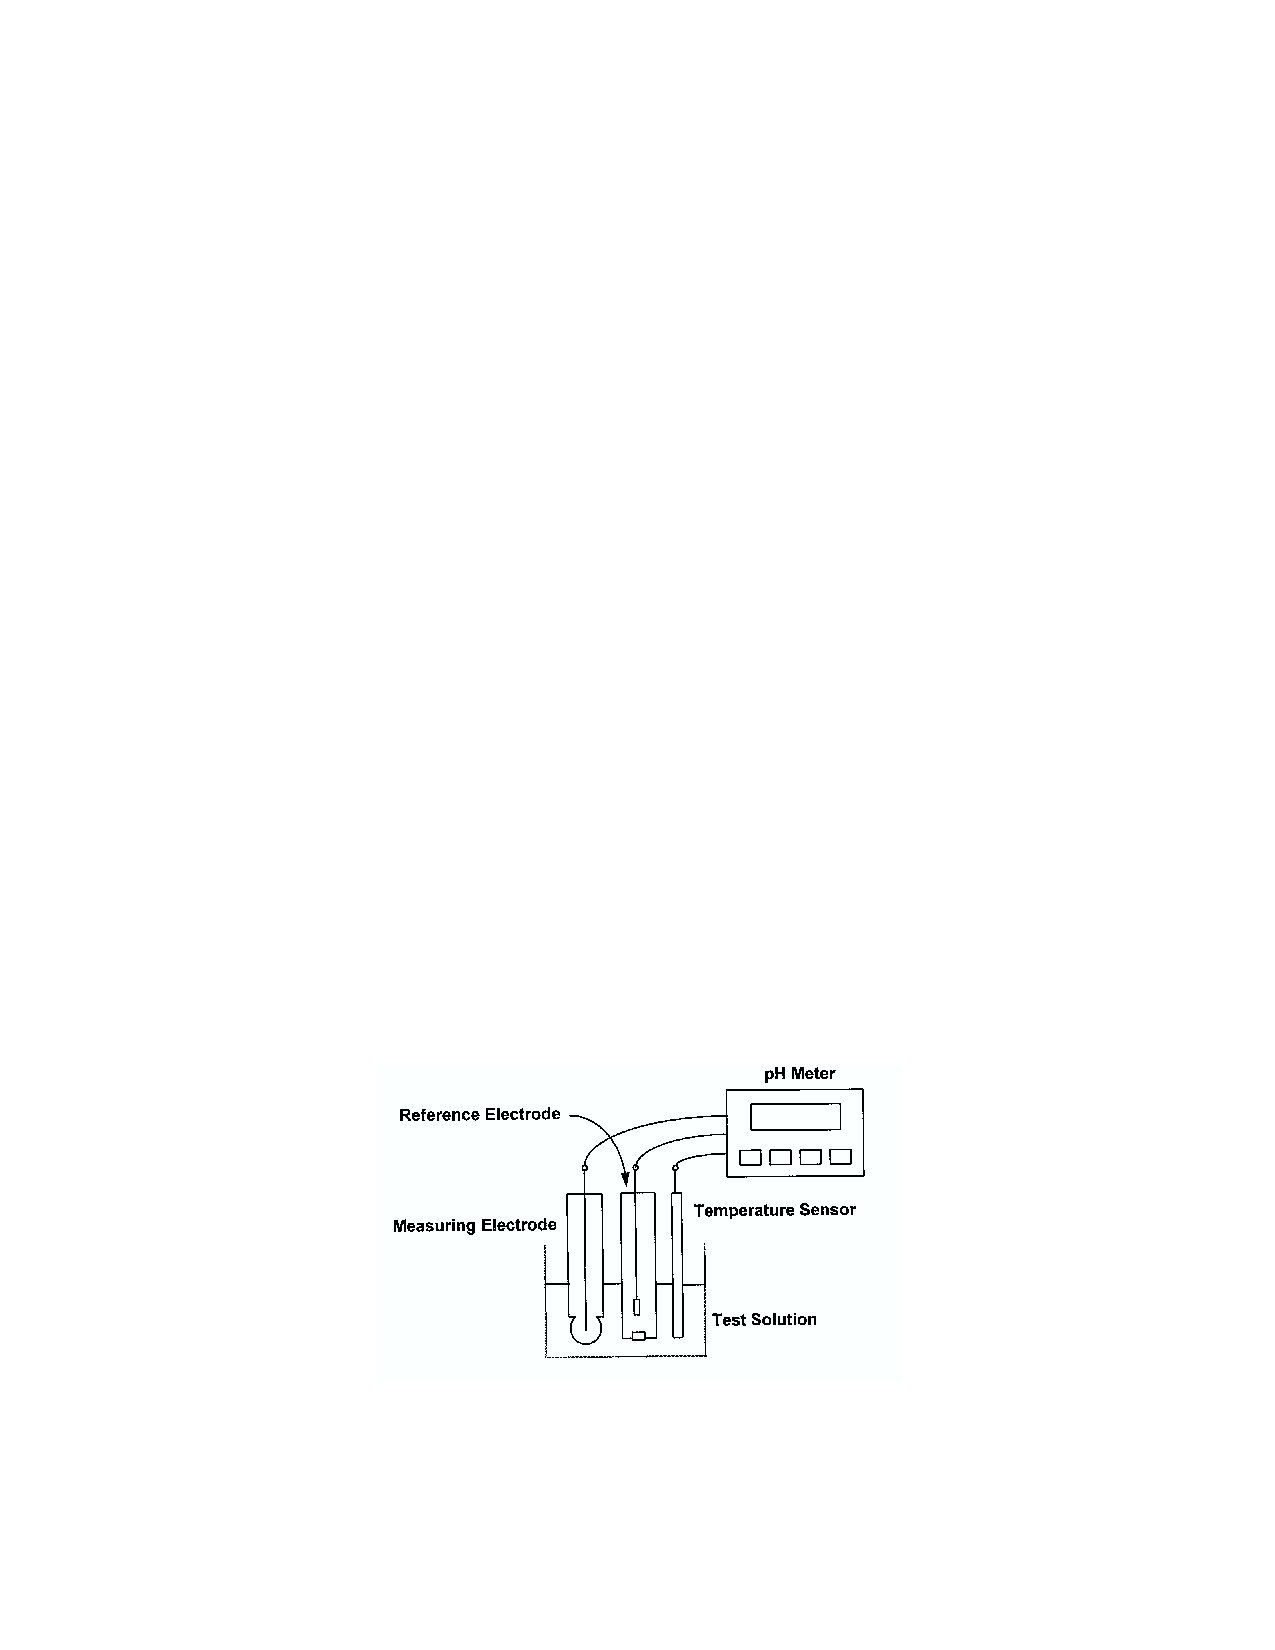
\includegraphics[scale=1]{diagrama-ph.pdf}
	\end{center}
	\caption{Esquema simplificado del medidor de pH.}
	\label{fig1}
\end{figure}

\clearpage

\section{Conversión de voltaje a pH}

La ecuación que relacióna la medición de tensión en la celda (mV), pH y temperatura (Kelvin) está dada por la siguiente expresión:

\begin{equation}
	E(T) = E^\circ - 0.1984\times T\times pH
\end{equation}

Donde $E^\circ$ es la suma de:

\begin{itemize}
	\item {El potencial correspondiente al electrodo de referencia.}
	\item {El potencia dentro de la superficie de la membrana de vidrio.}
	\item {El potencial de referencia externo.}
	\item {El potencial de la juntura líquida.}
\end{itemize}

El término $-0.1984\times T\times pH$, es el potencial (en mV) fuera de la superficie del vidrio del sensor. Este potencial depende de la temperatura y del pH en la muestra. Asumiendo que la temperatura permanece constante, cualquier cambio en la tensión de la celda está dado por el pH en la muestra. Por lo tanto, el voltaje obtenido de la celda electroquímica es una medida de pH correspondiente a la muestra. La transferencia típica de un celda electroquímica para medición de pH se puede observar en la Figura \ref{fig2}.

\begin{figure}[h!]
	\includegraphics[width=1\linewidth]{transferencia.eps}
	\captionof{figure}{Función transferencia de una celda electroquímica para medir pH.}
	\label{fig2}
\end{figure}

Teniendo en cuenta esto y que estas celdas tiene una alta impedancia de salida, podemos diseñar un sistema que muestre en display el valor de pH. El sistema de conversión propuesto consiste en tres pasos:

\begin{enumerate}
	\item {Realizar una adaptación de señales, tener en cuenta que la membrana de vidrio causa una resistencia interna de miles de M$\mathrm{\Omega}$.}
	\item {Enviar esta señal a un conversor Analógico-Digital, ya sea utilizando un integrado dedicado o implementando uno dentro de un microcontrolador.}
	\item {En caso de ser necesario, realizar una promediación de los valores para mejorar la resolución de la medición y mostrar el resultado en un display.}
\end{enumerate}

\clearpage

Por último, se plantean las siguientes especificaciones para el medidor:

\begin{itemize}
	\item{Rango de Medición: 0 - 14pH.}
	\item{Resolución: $\mathrm{\pm}$0,1pH.}
	\item {Rapidez de conversión de 1 palabra/segundo.}
\end{itemize}

Para ello se dispone del microcontrolador \texttt{Atmega 328p} que dispone de un CAD con las siguientes características:

\begin{itemize}
	\item{Conversor Analógico Digital de aproximaciones sucesivas.}
	\item {Resolución de 10 bits.}
	\item {Tiempo de conversión: 13 - 260 $\mathring{\mu S}$}
	\item {7690 Palabras por segundo.}
	\item{Voltage de entrada: 0 - $\mathrm{V_{CC}}$.}
	\item{Generación de interrupciones al finalizar una conversión.}
\end{itemize}

Y una celda química diseñada para realizar la medición \emph{(Fig. \ref{fig3})}

\begin{figure}[h!]
	\begin{center}
		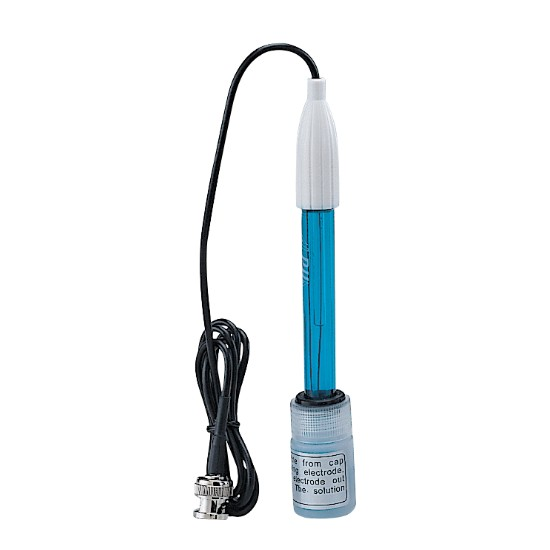
\includegraphics[scale=1.5]{celda-quimica.jpg}
	\end{center}
	\caption{Celda química para medir pH.}
	\label{fig3}
\end{figure}

\end{document}


